\documentclass[12pt,a4paper]{article}
\usepackage[utf8]{inputenc}
\usepackage[spanish]{babel}
\usepackage{amsmath}
\usepackage{amsfonts}
\usepackage{amssymb}
\usepackage{graphicx}
\usepackage[left=2cm,right=2cm,top=2cm,bottom=2cm]{geometry}
\author{Edwin Paez Guerrero }
\title{Informe de caracterización }
\begin{document}
tabla slew rate para los opams, average 600 [mV]

\begin{tabular}{|c|c|}
\hline 
\rule[-1ex]{0pt}{2.5ex} Elemento &  Slew Rate [V/$us$] \\ 
\hline 
\rule[-1ex]{0pt}{2.5ex} 1 & $9.83$ \\ 
\hline 
\rule[-1ex]{0pt}{2.5ex} 2 & $10.06$ \\ 
\hline 
\rule[-1ex]{0pt}{2.5ex} 3 & $10.17$ \\ 
\hline 
\rule[-1ex]{0pt}{2.5ex} promedio & $10.02$ \\ 
\hline 
\end{tabular} 

\begin{figure}
  \centering
    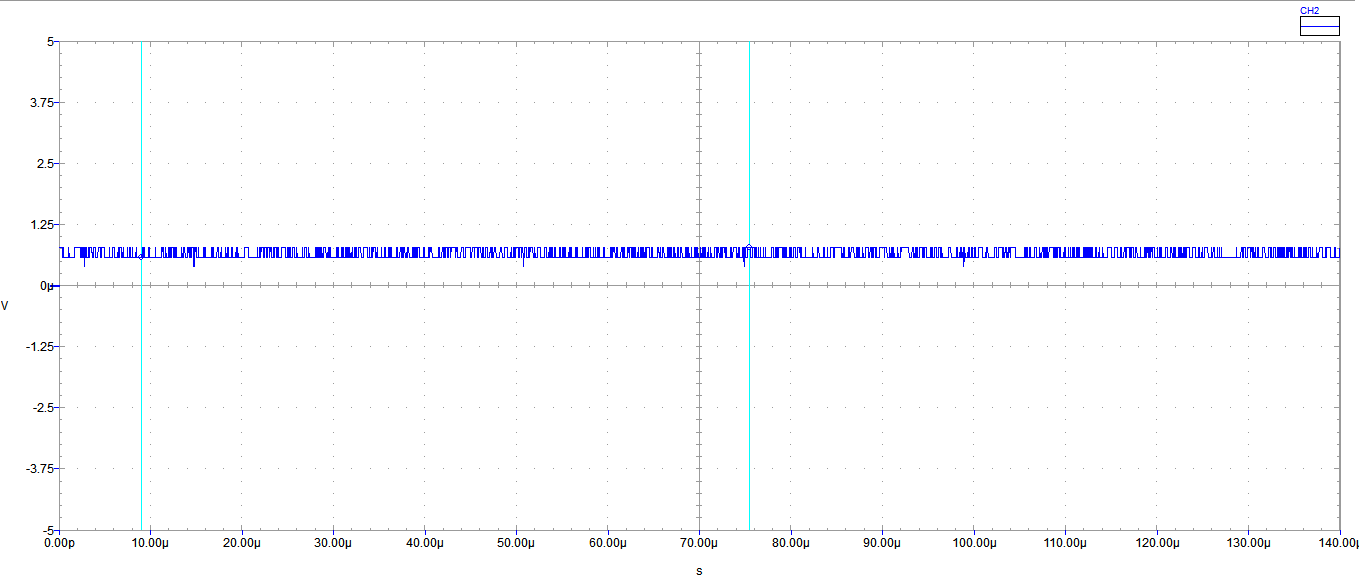
\includegraphics[width=0.5\textwidth]{average_opam.png}
  \caption{Average del opam}
  \label{fig:ejemplo}
\end{figure}

\begin{figure}
  \centering
    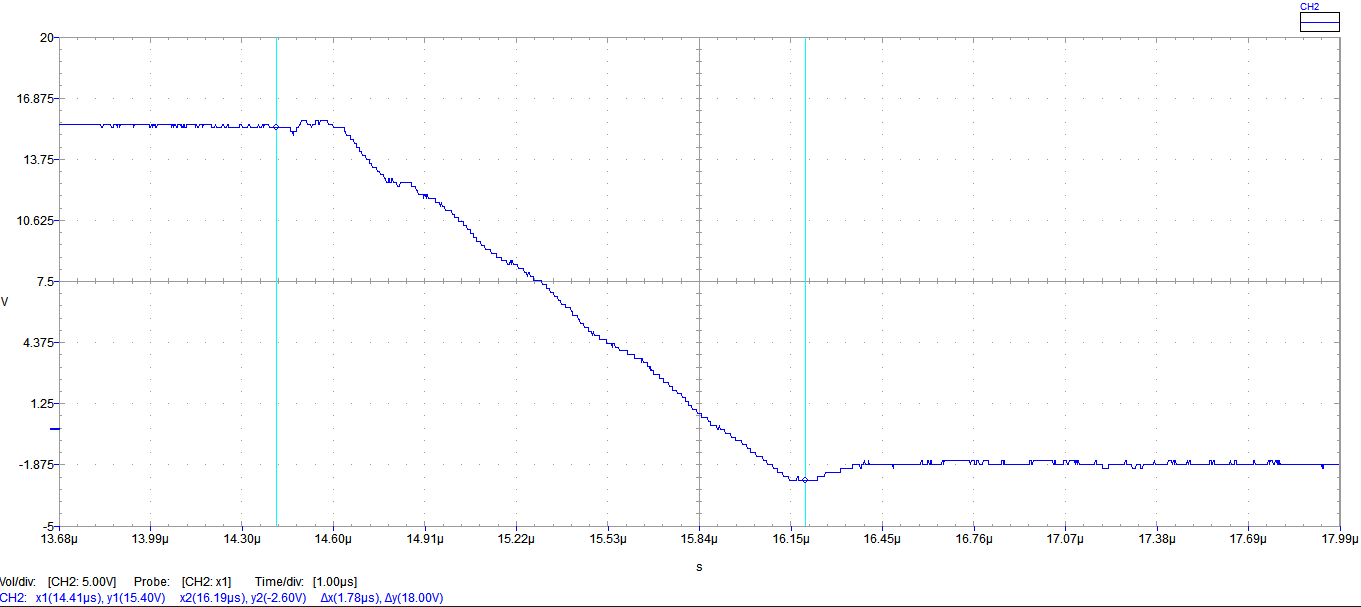
\includegraphics[width=0.5\textwidth]{slew_rate_opam.png}
  \caption{slew rate opam}
  \label{fig:ejemplo}
\end{figure}

\end{document}